\chapter{Evaluation}
\label{ch:Evaluation}

In the previous chapters we:
\begin{enumerate}
    \item Described the results of our single-threaded PageRank microbenchmark using different Vertex-and-Edge ordering combinations. We saw that specific Vertex-and-Edge orderings (e.g. Slashburn Vertex Order and Hilbert Edge Order) consistently yielded the greatest speedup. This motivated us to parallelize the SlashBurn Vertex Reordering algorithm.
    \item Described the Parallel SlashBurn algorithm and evaluated how well it scales by increasing the number of cores.
          \AT{I think it makes sense to discuss and show the evaluation of how well Parallel Slashburn scales right after I describe how I've implemented it - i.e. at the end of that chapter}.
    \item Described and analyzed RHuBarb (Recursive Hilbert Blocking).
\end{enumerate}

Now, we answer the following Research Questions:

\begin{itemize}
    \item [\textbf{RQ1}] \textit{How expensive is RHuBarb's preprocessing?}
          \begin{itemize}
              \item [\textbf{RQ1.1}] RHuBarb benefits from compressed graph representations (those with a \textit{smaller} number of \textit{denser} blocks, as opposed to a \textit{larger} number of \textit{sparser} blocks.) \textbf{How long do these vertex reorderings take to compute?}
              \item [\textbf{RQ1.2}]{ \textbf{How long does RHuBarb's divide-and-conquer blocking algorithm take?}}
              \item [\textbf{RQ1.3}] \textbf{How well does RHuBarb's divide-and-conquer blocking algorithm scale with an increasing number of cores?}
          \end{itemize}
    \item [\textbf{RQ2}] \textbf{How does RHuBarb compare to State-of-the-Art Graph Processing Systems (GPS)?}
          \AT{This will involve an evaluation of:}
          \begin{enumerate}
              \item Systems: GPOP, Syze, Ligra, GraphMat.
              \item Graphs:
                    \begin{itemize}
                        \item Social Networks: Twitter, Twitter-MPI, Friendster.
                        \item Hyperlink Networks: UK Domain, Wikipedia.
                        \item Road Networks: US Road Network.
                        \item Bipartite User-Item Rating Networks (Specific to Collaborative Filtering benchmark): Yahoo Songs, Amazon.
                    \end{itemize}
              \item Edge-Centric Algorithms:
                    \begin{itemize}
                        \item PageRank, Connected Components, Collaborative Filtering.
                    \end{itemize}
          \end{enumerate}
    \item [\textbf{RQ3}] The performance of RHuBarb depends on 2 user-defined parameters:
    \begin{enumerate}
        \item \textit{$d$, Dynamic Group Size}: How many consecutive Hilbert blocks should be dynamically assigned to cores during Edge-Centric traversal?
        \item \textit{$m$, Maximum Number of Edges per Block}: each Hilbert block must contain \textit{at most} this many edges. 
    \end{enumerate}
    \textbf{How should users choose the values for $d, m$?}
    \item [\textbf{RQ4}] In answering \textbf{RQ2}, we identified a performance bottleneck for SOTA systems (GPOP, SYZE) on graphs whose vertices have been relabelled using the SlashBurn or Descending Degree Sort vertex reorderings (i.e. graphs with ``concentrated edge densities''). Since, given an arbitary input graph, one has no a priori knowledge of the edge density of the graph's ``Original'' vertex ID assignment (except for known examples of Hyperlink networks in the literature), we answer the following:
    \textbf{For graphs whose ``Original'' Vertex ID assignment is ``close'' to a Descending Degree Sort, does RHuBarb perform well out-of-the-box?}\\
    \AT{Or maybe?}
    \textbf{How often are the Vertex IDs of real-world graphs close to a Descending Degree Sort?}
\end{itemize}

We begin this chapter by describing the GPS we'll compare against and the graph datasets and algorithms we'll use in our comparison.
Table \ref{Tab:datasets} lists the graph datasets we used in our evaluation and Sections \ref{sec:ec-algos} and \ref{sec:ggps} briefly describe the algorithms and systems, respectively, and why we chose these specifically.
\crefname{section}{Section}{Sections} % capitalize "E", no period
\crefrangelabelformat{section}{(#3#1#4--#5#2#6)}
\crefrange{sec:preproc}{sec:rank-compare} answer \textbf{RQ1-4}, respectively.

\begin{table}[ht]
    \caption{Graph Datasets}
    \centering
    \hspace*{-2cm}
    \begin{tabular}{ |c| c| c| c | }
        \hline
        Graph            & Description      & $n$        & $m$           \\
        \hline
        \textit{twitter} & Twitter Follower & 41,652,230 & 1,468,365,182 \\
        \hline
        \textit{road} & USA Road & 23,947,347  & 57,708,624  \\
        \hline
        \textit{uk} & Hyperlink Network of .uk Domain & 105,153,952   & 3,301,876,564   \\
        \hline
        \textit{amazon} & Rating Network & 31,050,733    & 82,677,131    \\
        \hline
        \ldots & \ldots & \ldots & \ldots \\
        \hline
    \end{tabular}
    \label{Tab:datasets}
\end{table}





\section{Edge-Centric Graph Algorithms}\label{sec:ec-algos}
\subsection{PageRank}
\subsection{Connected Components}
\subsection{Collaborative Filtering}
\section{Graph Frameworks}\label{sec:ggps}
\subsection{Ligra}
\subsection{GraphMat}
\subsection{GPOP and Syze}

\section{Preprocessing Overhead}\label{sec:preproc}
This section lists the preprocessing time of various vertex reorderings 
\AT{Parallel-SlashBurn, Descending Degree Sort, Degree-Based-Grouping, Rabbit Order, COrder}and Recursive Hilbert-Blocking. We find that certain costly vertex reorderings take longer to compute than certain graph algorithms. In such cases, we also list the number of times the computation must be repeated to amortize the total cost of preprocessing.

\subsection{Cost of Vertex Reorderings}
\subsection{Cost of Recursive Hilbert-Blocking}
\subsection{Scaling of Recursive Hilbert-Blocking}
\subsection{Time to Amortize Costly Preprocessing Steps}
\section{Multicore Comparison} \label{sec:multicore}
This section compares RHuBarb to State-of-the-Art, main-memory GPS.
We compare the performance of RHuBarb to these systems using a representative set of Edge-Centric graph algorithms and graph datasets. Using an increasing number of cores, we measure runtime performance and L2 and LLC cache miss rate.

\AT{A figure like \ref{fig:eval-sample} for PageRank, Connected Components, and Collaborative Filtering. 
(More coloured lines to show the performance of the different systems.)
Also, similar figures to show the L2, LLC Cache-miss rates as we increase the number of cores.
}
\begin{figure}[!htb]
    \centering
    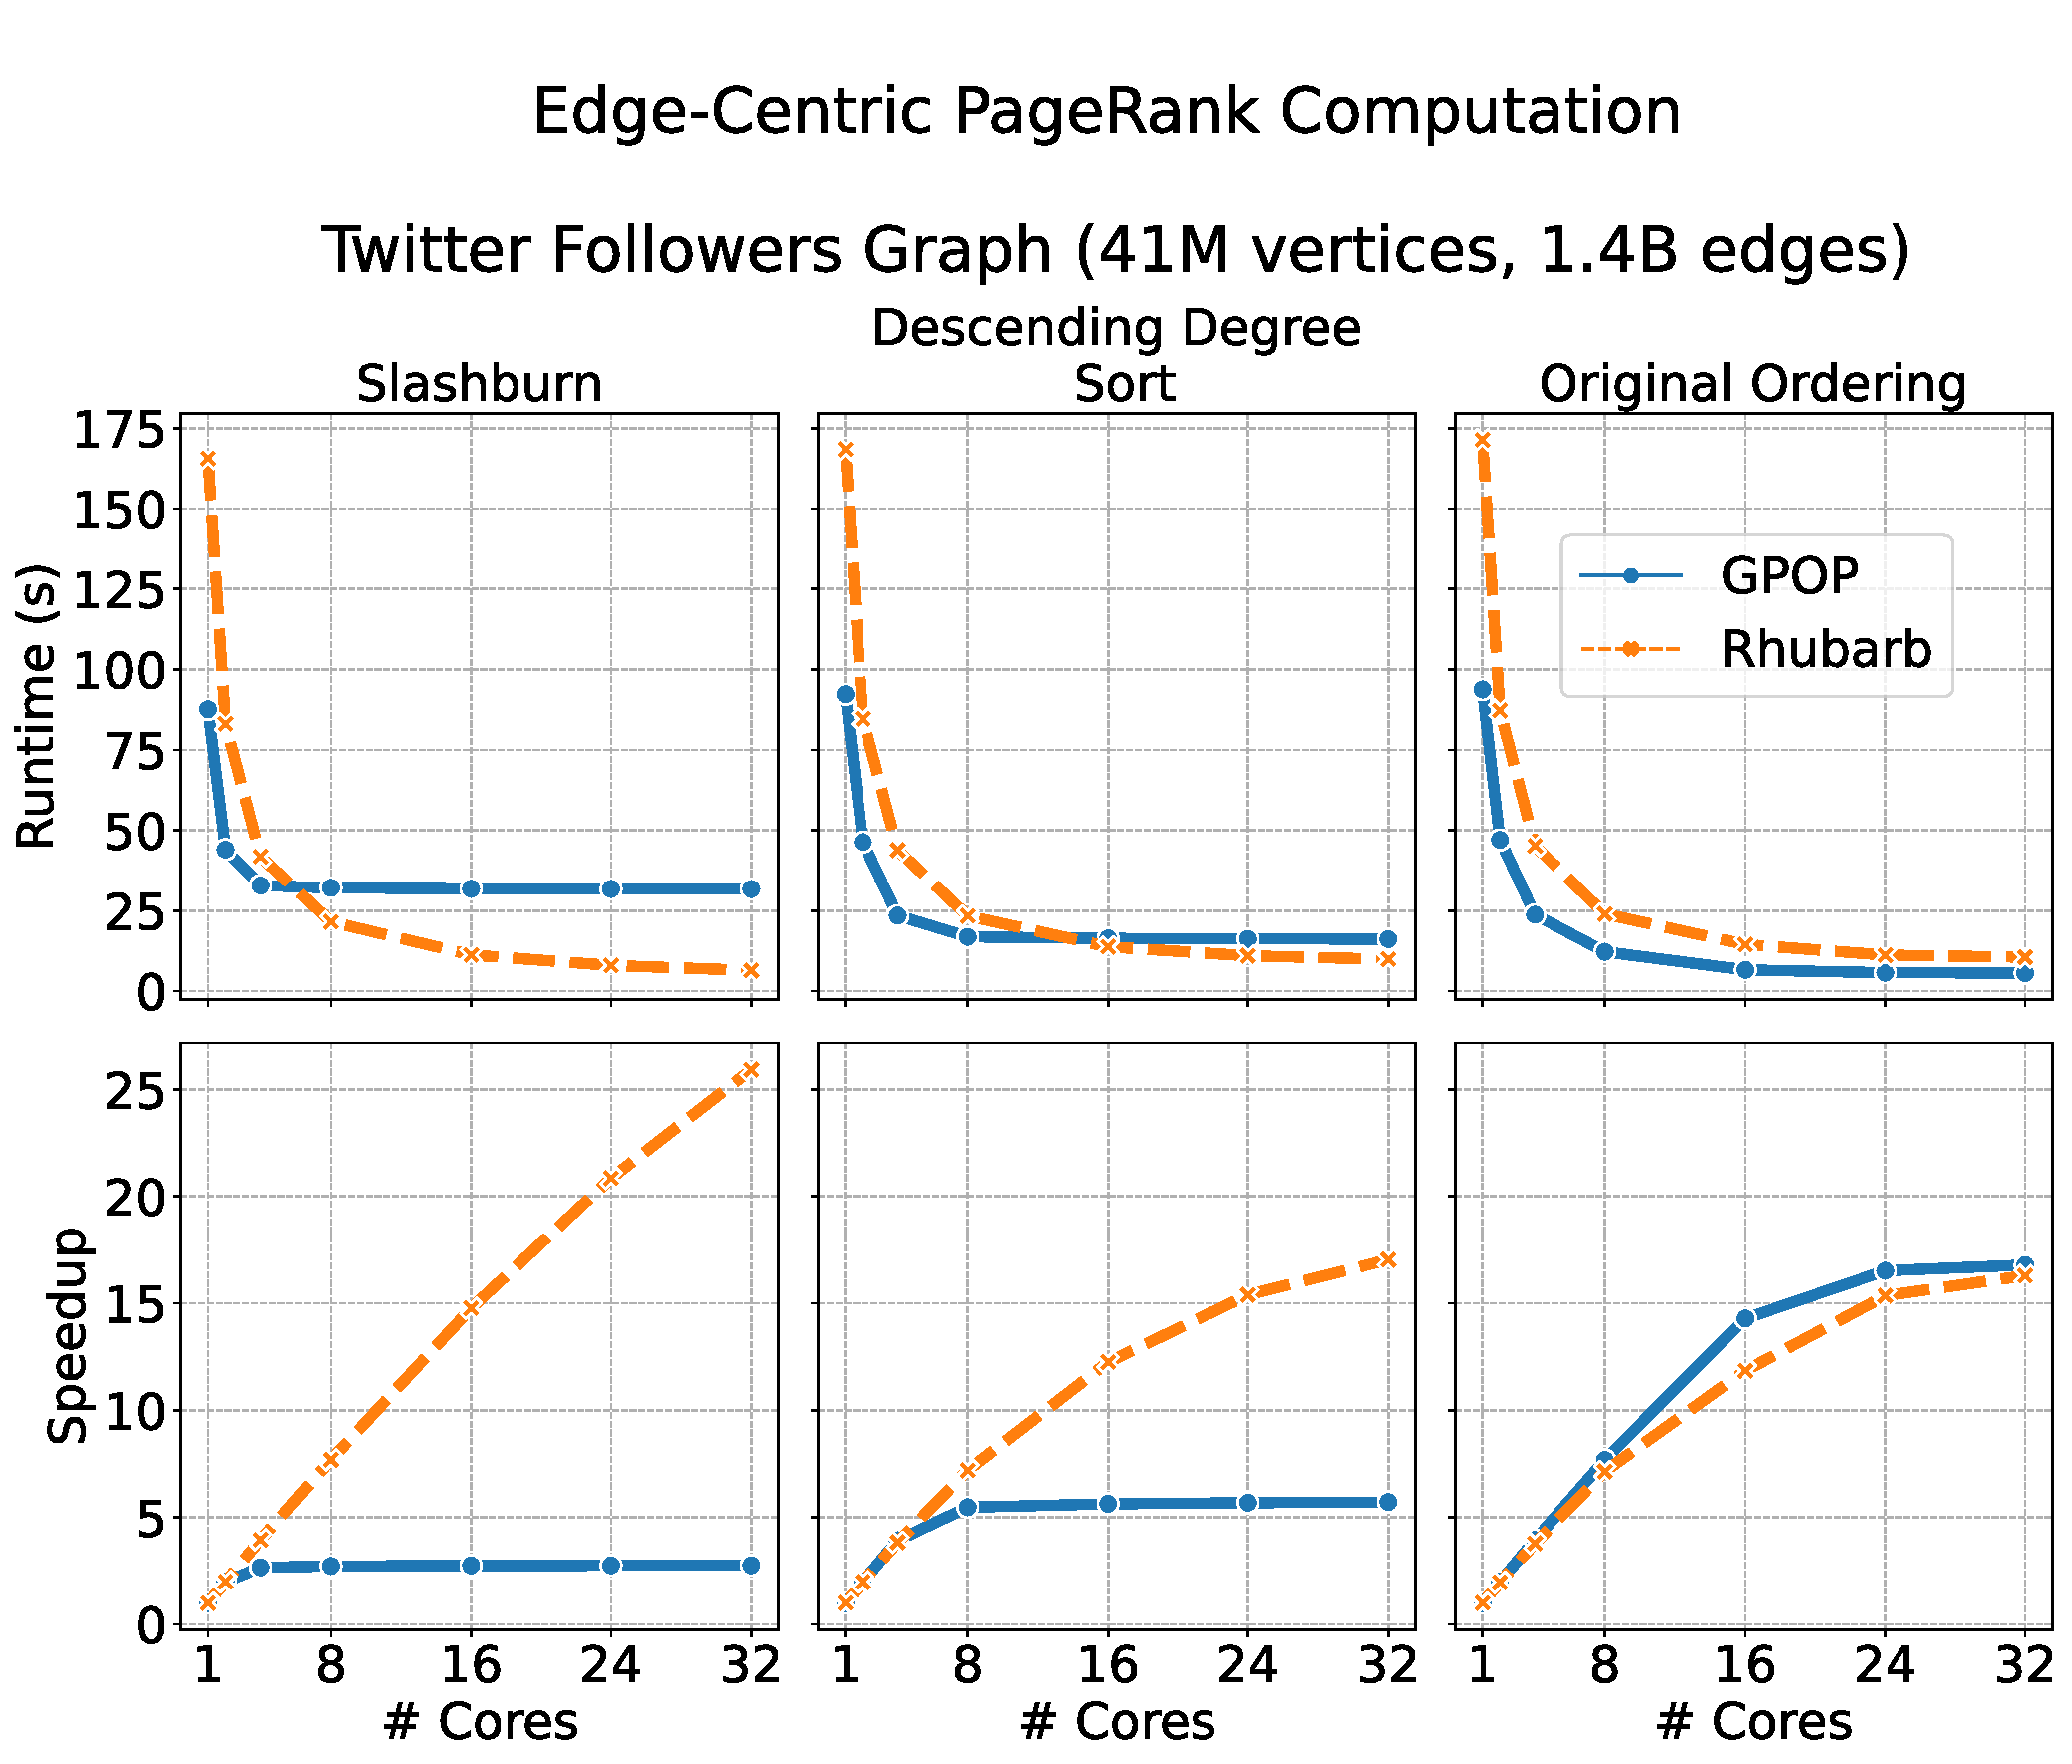
\includegraphics[width=5in]{plots/eval/twitter-sample.pdf}
    % \includesvg[width=5in]{plots/eval/twitter-sample.svg}
    \caption{Runtime and Scaling for different vertex reorderings (Original, Descending (Out) Degree Sort, and  Slashburn) for PageRank computation using GPOP and Hilbert Blocking.}
    \label{fig:eval-sample}   % label should change
    \end{figure}

\section{Effect of Dynamic Group Size and Minimum Number of Edges per Block}\label{sec:hparams}

In this section, we evaluate the effect of the 2 user-defined parameters of RHuBarb on  performance.

\begin{enumerate}
    \item \textit{$d$, Dynamic Group Size}: How many consecutive Hilbert blocks should be dynamically assigned to cores during Edge-Centric traversal?
    \item \textit{$m$, Maximum Number of Edges per Block}: each Hilbert block must contain \textit{at most} this many edges. 
\end{enumerate}

We perform this performance analysis in order to find a heuristic value for these user-defined parameters.
We evaluate RHuBarb using the combination of $d\in\{1, 2, 4, 8, 16, 32, 64\}$ and 
$m\in\{
    \num[group-separator={,}]{8192}, 
    \num[group-separator={,}]{16384}, 
    \num[group-separator={,}]{32768}, 
    \num[group-separator={,}]{65536}, 
    \num[group-separator={,}]{131072}, 
    \num[group-separator={,}]{262144}
\}$.

Since the combination of $d$ and $m$ dictates the amount of work assigned to each core, we find that the size of the private L2 Cache acts as a good heuristic for a rough upper bound of values to assign to $d$ and $m$. As a result, RHuBarb uses the L2 cache-size at runtime to assign values to $d$ and $m$.

\section{On which graphs does RHuBarb perform well ``out-of-the-box''?}\label{sec:rank-compare}

          \AT{ This is the ``fuzziest'' section in my mind, and is my attempt to answer your note about ``Default orders'' in your email response. I'm not sure how useful the distance metrics I found are for the purpose of comparing the similarity between two vertex reorderings. My current hypothesis is the following:
          }
          \begin{enumerate}
            \item I observed that RHuBarb outperformed SOTA on specific graphs \textbf{without} performing any vertex reordering (i.e. using the original vertex ID assignment). 
            \item I hypothesize that, for these graphs, the ``distance'' between the ``Original'' order and a Descending Degree Sort should be \textbf{smaller} than the distance between Original and Descending Degree Sort for graphs for which we \textit{did} need to sort them to see any performance improvement using RHuBarb.
          \end{enumerate}

          \AT{The distance metrics I'm considering:}
          \begin{itemize}
            \item \textbf{Weighted Kendall Tau Distance}: measures the number of pairwise disagreements between two rankings. It counts the number of times that two items are ranked differently between two rankings. \AT{I can weigh vertex rankings by the vertices' out-degrees. i.e. Vertices with high degrees will contribute more to the final distance scores than vertices with low degree. I don't think this is a good metric, because it simply counts the number of times vertex ID assignment were out of order, not ``how'' out of order they were. For this reason, I think Manhattan distance (below), makes more sense.}
            \item \textbf{Manhattan distance}: calculates the distance between two rankings based on the sum of the absolute differences between the ranks of each vertex.
          \end{itemize}

% \end{document}

